\chapter{Gaia-X}\label{ch:gaiax}

\begin{chapterabstract}
    In this chapter, we will introduce reader to the initiative \textbf{Gaia-X}.
    We will go over its vision, the means to achieve them, their target organizations and how it may help projects like \textbf{Carecentive}.
\end{chapterabstract}

\section{About Gaia-X}\label{sec:about-gaia-x}

The \textbf{Gaia-X} is the initiative led by the ``Gaia-X Association AISBL'' organization.
The association was registered as an \textit{international non-profit association} \textit{(French: Association Internationale sans but lucratif)} in Belgium in January 2021 and is funded privately.
It was founded by \textit{22} companies and organizations in \textit{January 2021}, but at the time of writing (January 2024), the association has over \textit{350} members from backgrounds like data infrastructure providers, IT startups research institutions and business associations. % TODO: update before completing the thesis
Additionally, representatives from business, politics, academia, research, technology, policy, government, and science from Europe and beyond cooperate with the \textit{Gaia-X Association AISBL} in their mission.
The association claims to have no business interest.~\cite{gaiax}

\section{The Goal}\label{sec:gaia-x-goal}

The goal of the \textbf{Gaia-X} initiative is to enable exchange of data in a \textit{safe} and \textit{trustworthy} environment.
The coveted outcome is a federated system connecting many cloud service providers and users together in an environment that is \textit{interoperable} \textit{transparent}, \textit{open}, \textit{secure}, and respects \textit{data rights} and \textit{EU regulations}.~\cite{gaiax}

\section{The structure}\label{sec:the-structure}

The organisational structure of the ``Gaia-X Association AISBL'' is well-defined and transparent.
The topmost body of the \textit{association} is the \textbf{General Assembly}.
It is composed of all the members of the \textit{association} and has complete authority to carry out the objectives of the \textit{Gaia-X initiative}.~\cite{gaiax}

Under the \textbf{General Assembly} are the boards \em \textit{Governmental Advisory Board}, \textit{General Advisory Board} and the \textit{Board of Directors}.
The \textbf{Board of Directors} is elected by the \textbf{General Assembly} and is headed by a Chairperson and Vice-Chairperson. % TODO: find out how the General Advisory Board and the Governmental Advisory Board are selected
Its purpose is to decide on important matters regarding the \textit{Gaia-X Association}.~\cite{gaiax} % TODO: clarify what the 'important matters' are?

Next up is the \textbf{Management Board} and its chairs \em \textit{Policy Rules Committee}, \textit{Data Spaces Business Committee}, and the \textit{Technical Committee}.
Each of the committees also has its own \textit{Working Group}.
The \textbf{Management Board} is appointed by the \textit{Board of Directors} and is composed of the Chief Executive Officer (CEO), the Chief Operating Officer (COO), the Chief Technical Officer (CTO), the Digital Communications Director and the Head of Finance and Administration.
Its purpose is the management of daily activities of \textit{Gaia-X Association}.~\cite{gaiax}

\begin{figure}
    \centering
    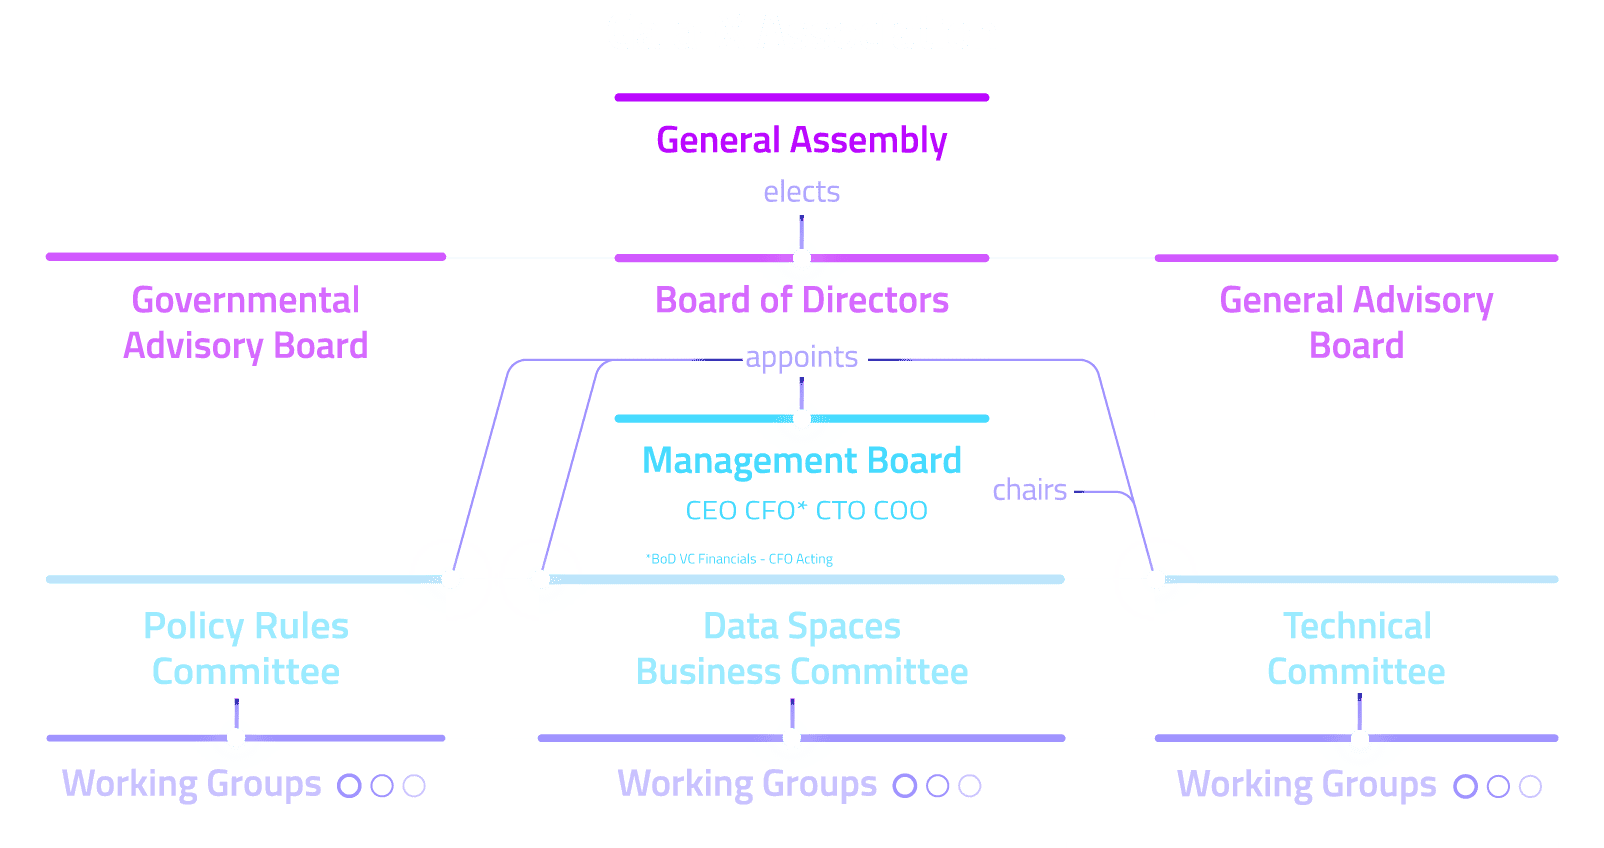
\includegraphics[width=\textwidth]{assets/management-board-structure}
    \caption{~Organisational structure of the Gaia-X Association~\cite{gaiax}}\label{fig:organisational-board-structure}
\end{figure}

\subsection{Data Spaces Business Committee}\label{subsec:data-spaces-business-committee}

The \textit{Data Spaces Business Committee (DSBC)} focuses on collecting \textit{economic}, \textit{functional}, \textit{operational} and \textit{legal} requirements that facilitate seamless collaboration and interconnection between \textit{Data Spaces}, \textit{Ecosystems}, \textit{Lighthouse Projects} and respective \textit{Hubs}. % FIXME: Data Spaces, Ecosystems, Lighthouse Projects and Hubs not defined yet
Furthermore, the \textit{DSBC} supports the creation of Data Spaces by third parties across Europe and beyond.~\cite{gaiax}

\subsection{Policy Rules Committee}\label{subsec:policy-rules-committee}

The \textit{Policy Rules Committee (PRC)} exists to translate the guiding principles of the Gaia-X initiative (\textit{transparency}, \textit{data protection}, \textit{cyber-security}, \textit{portability}, \textit{openness},~\ldots) into High-Level Objectives and to preserve the added value of the \textit{Gaia-X ecosystem}.
The additional role of the \textit{PRC} is to monitor, integrate and define the relationship with EU regulations and external standards.
The Committee guides and delivers the \textit{Gaia-X Trust Framework}, \textit{Gaia-X Policy Rules and Labelling Document} (formerly Policy Rules Document and Gaia-X Labelling Criteria).
These deliverables are provided by the Committee's three \textit{Working Groups} (WG).~\cite{gaiax}
\begin{itemize}
    \item \textbf{Labels \& Qualification} WG:~provides the \textit{Gaia-X Labelling Framework} and prepares the ``Gaia-X Policy Rules and Labelling Document'' together with the \textit{Policy Rules Document} WG
    \item \textbf{Policy Rules Document} WG:~defines \textit{High-Level Objectives} and prepares the ``Gaia-X Policy Rules and Labelling Document'' together with the \textit{Policy Rules Document} WG
    \item \textbf{Compliance} WG:~provides the \textit{Gaia-X Trust Framework}, representing the reference document for the Gaia-X compliance, providing the compulsory set of rules of the Gaia-X Ecosystem
\end{itemize}

\subsection{Technical Committee}\label{subsec:technical-committee}

The purpose of the \textit{Technical Committee (TC)} is to define and implement the technological vision of the \textit{Gaia-X initiative}.
It is in charge of transforming the high-level objectives of Gaia-X and requirements collected from other Committees and Gaia-X members into the \textit{technology roadmap} and is accountable for its contributors.
The Committee drafts and delivers the Gaia-X \textit{Architecture Document}, \textit{technical specifications} and related \textit{reference implementation}.
These deliverables are provided by the Committee's two \textit{Working Groups} (WG).~\cite{gaiax}
\begin{itemize}
    \item \textbf{Architecture} WG:~drafts the ``Gaia-X Architecture Document'', which describes the founding concepts of the \textit{Gaia-X Ecosystem}
    \item \textbf{Service Characteristics} WG:~specifies the Schema for the Self-Descriptions of Providers, their Service Offerings, and the Resources they are composed of
\end{itemize}

\begin{figure}
    \centering
    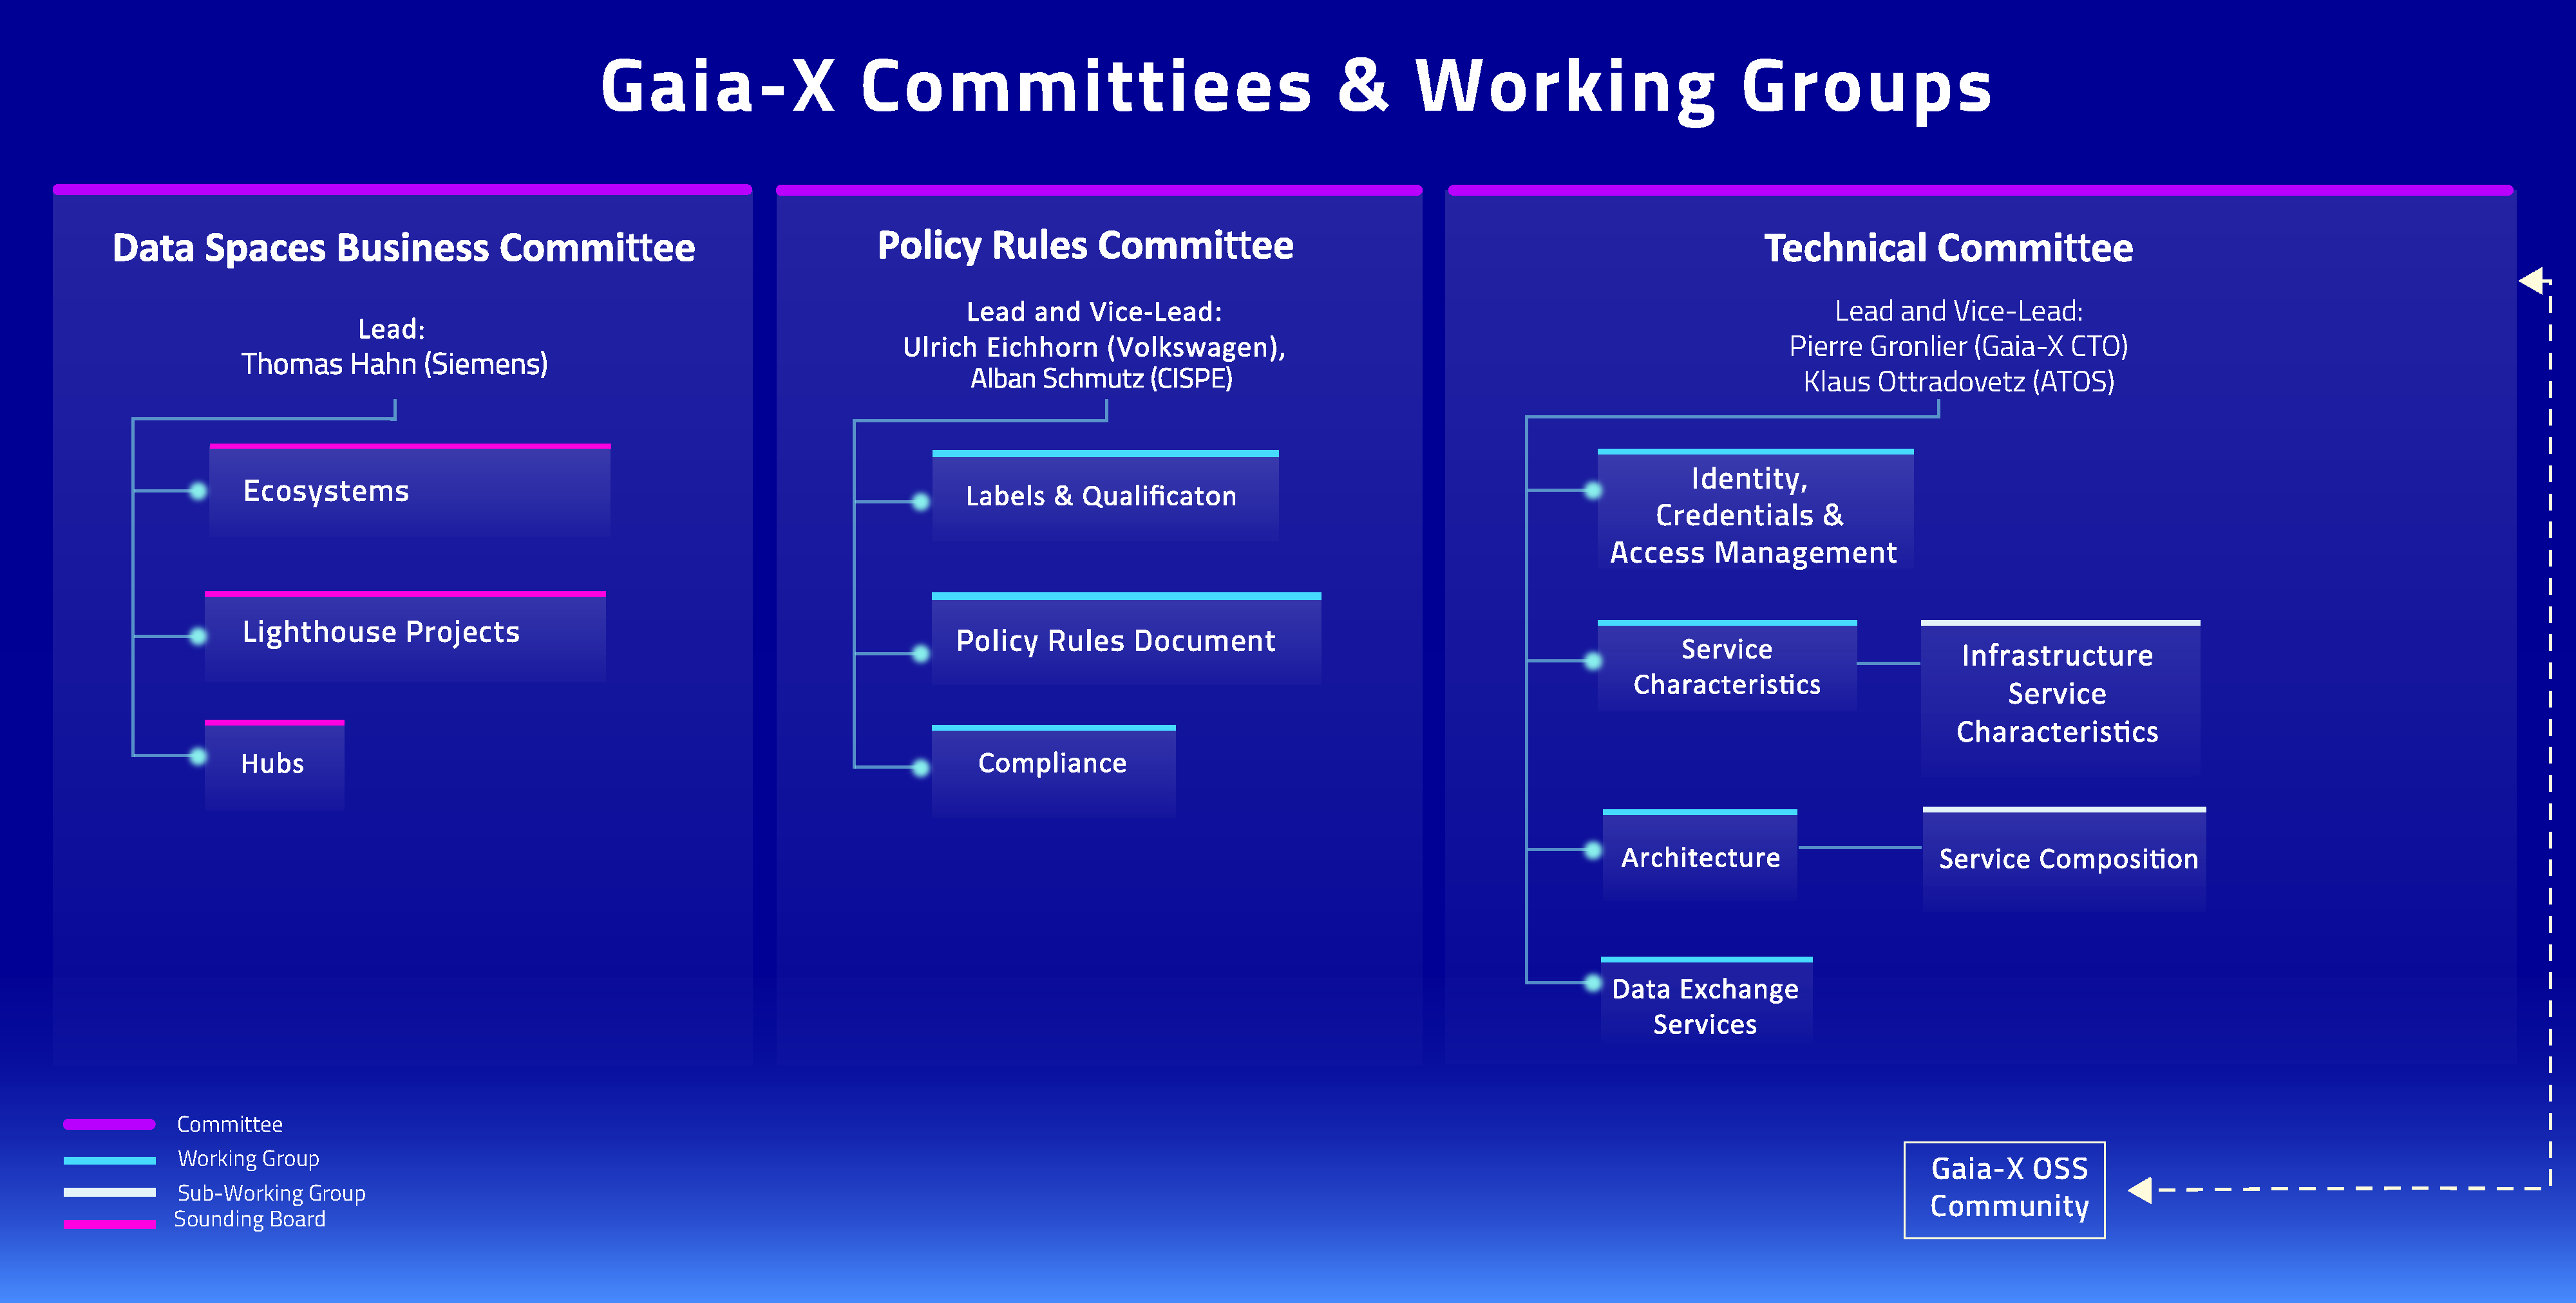
\includegraphics[width=\textwidth]{assets/committees-and-working-groups}
    \caption{~Organisational structure Committees and their Working Groups~\cite{gaiax}}\label{fig:organisational-committees-structure}
\end{figure}

\begin{figure}
    \centering
    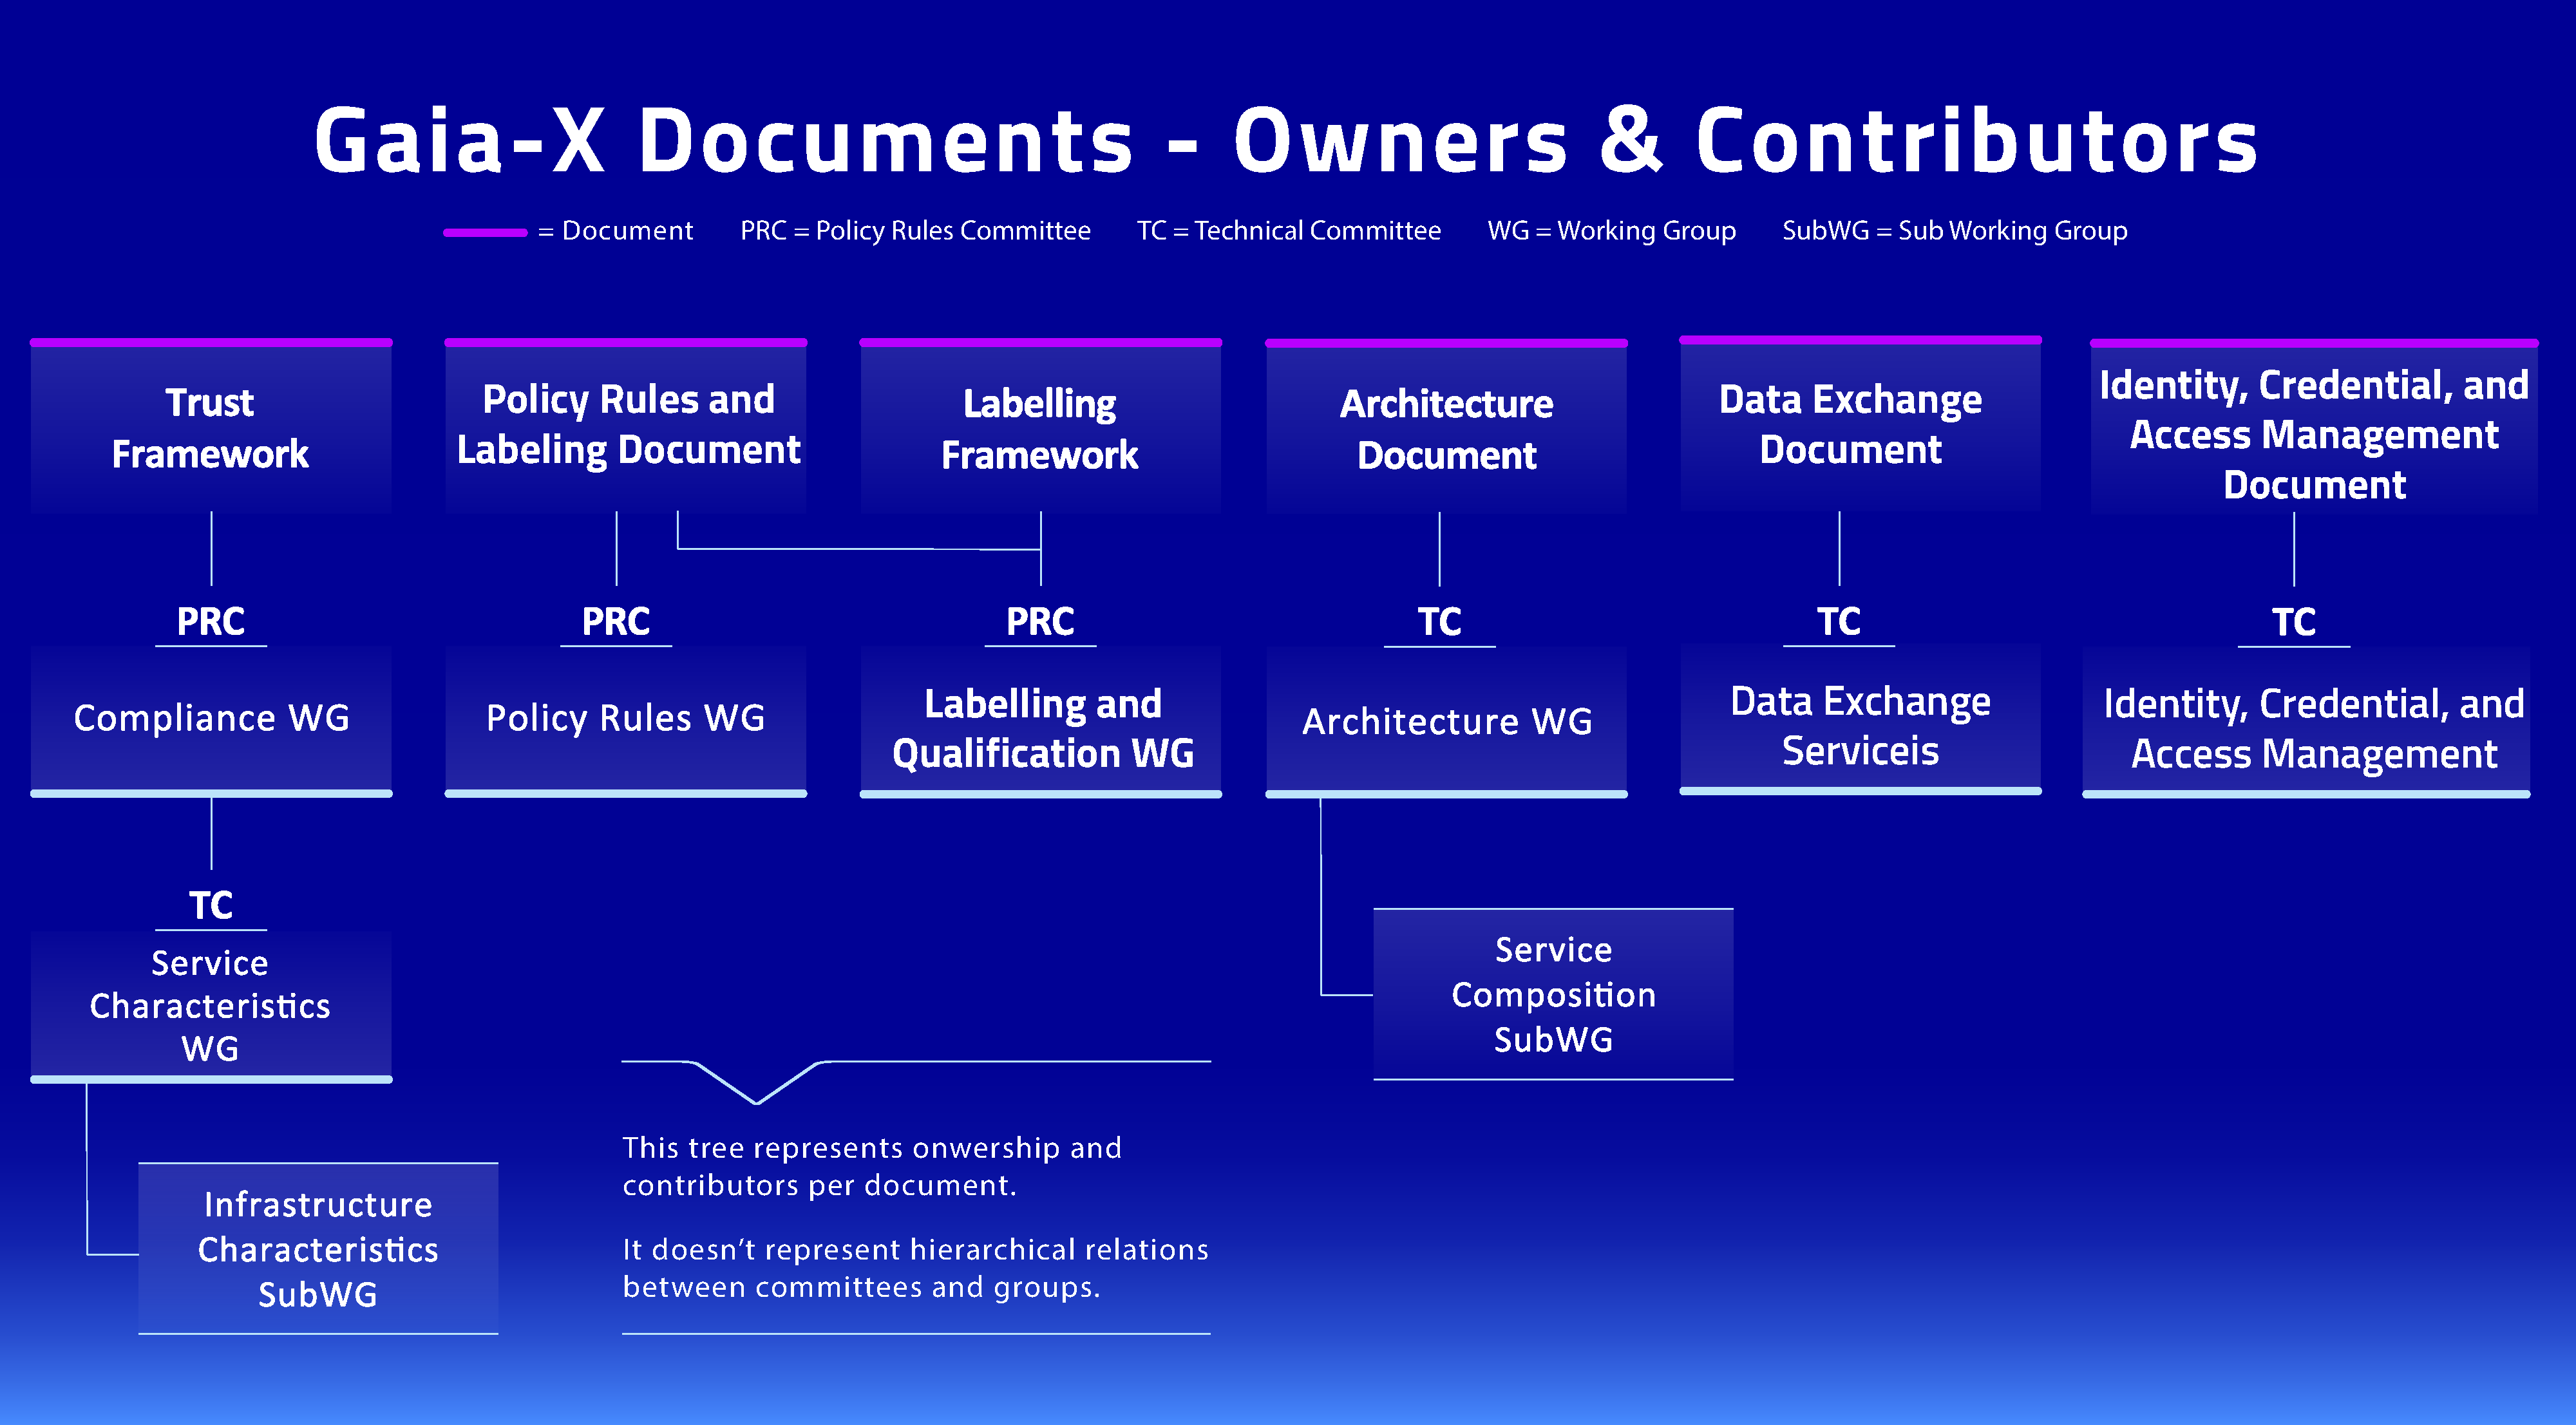
\includegraphics[width=\textwidth]{assets/committees-owners-and-contributors}
    \caption{~Gaia-X Documents - Owners \& Contributors~\cite{gaiax}}\label{fig:gaiax-documents-owners-and-contributors}
\end{figure}

% TODO: describe ecosystems and hubs

\section{Gaia-X Framework}\label{sec:gaia-x-framework}

These are categorized into three broad pillars: % this regards to Gaia-X framework (realization of goals)
\begin{itemize}
    \item Compliance:
    \item Federation:
    \item Data exchange:
\end{itemize}




% TODO: describe tthe trust framework
